\documentclass[tikz,border=3.14mm]{standalone}
\usepackage{tikz}
\usetikzlibrary{shapes.geometric, arrows.meta, positioning}

\tikzset{
    startstop/.style = {rectangle, rounded corners, minimum width=3cm, minimum height=1cm, text centered, draw=black, fill=red!30},
    process/.style = {rectangle, minimum width=3cm, minimum height=1cm, text centered, draw=black, fill=orange!30},
    decision/.style = {diamond, minimum width=3cm, minimum height=1cm, text centered, draw=black, fill=green!30},
    arrow/.style = {thick, -Stealth}
}

\begin{document}
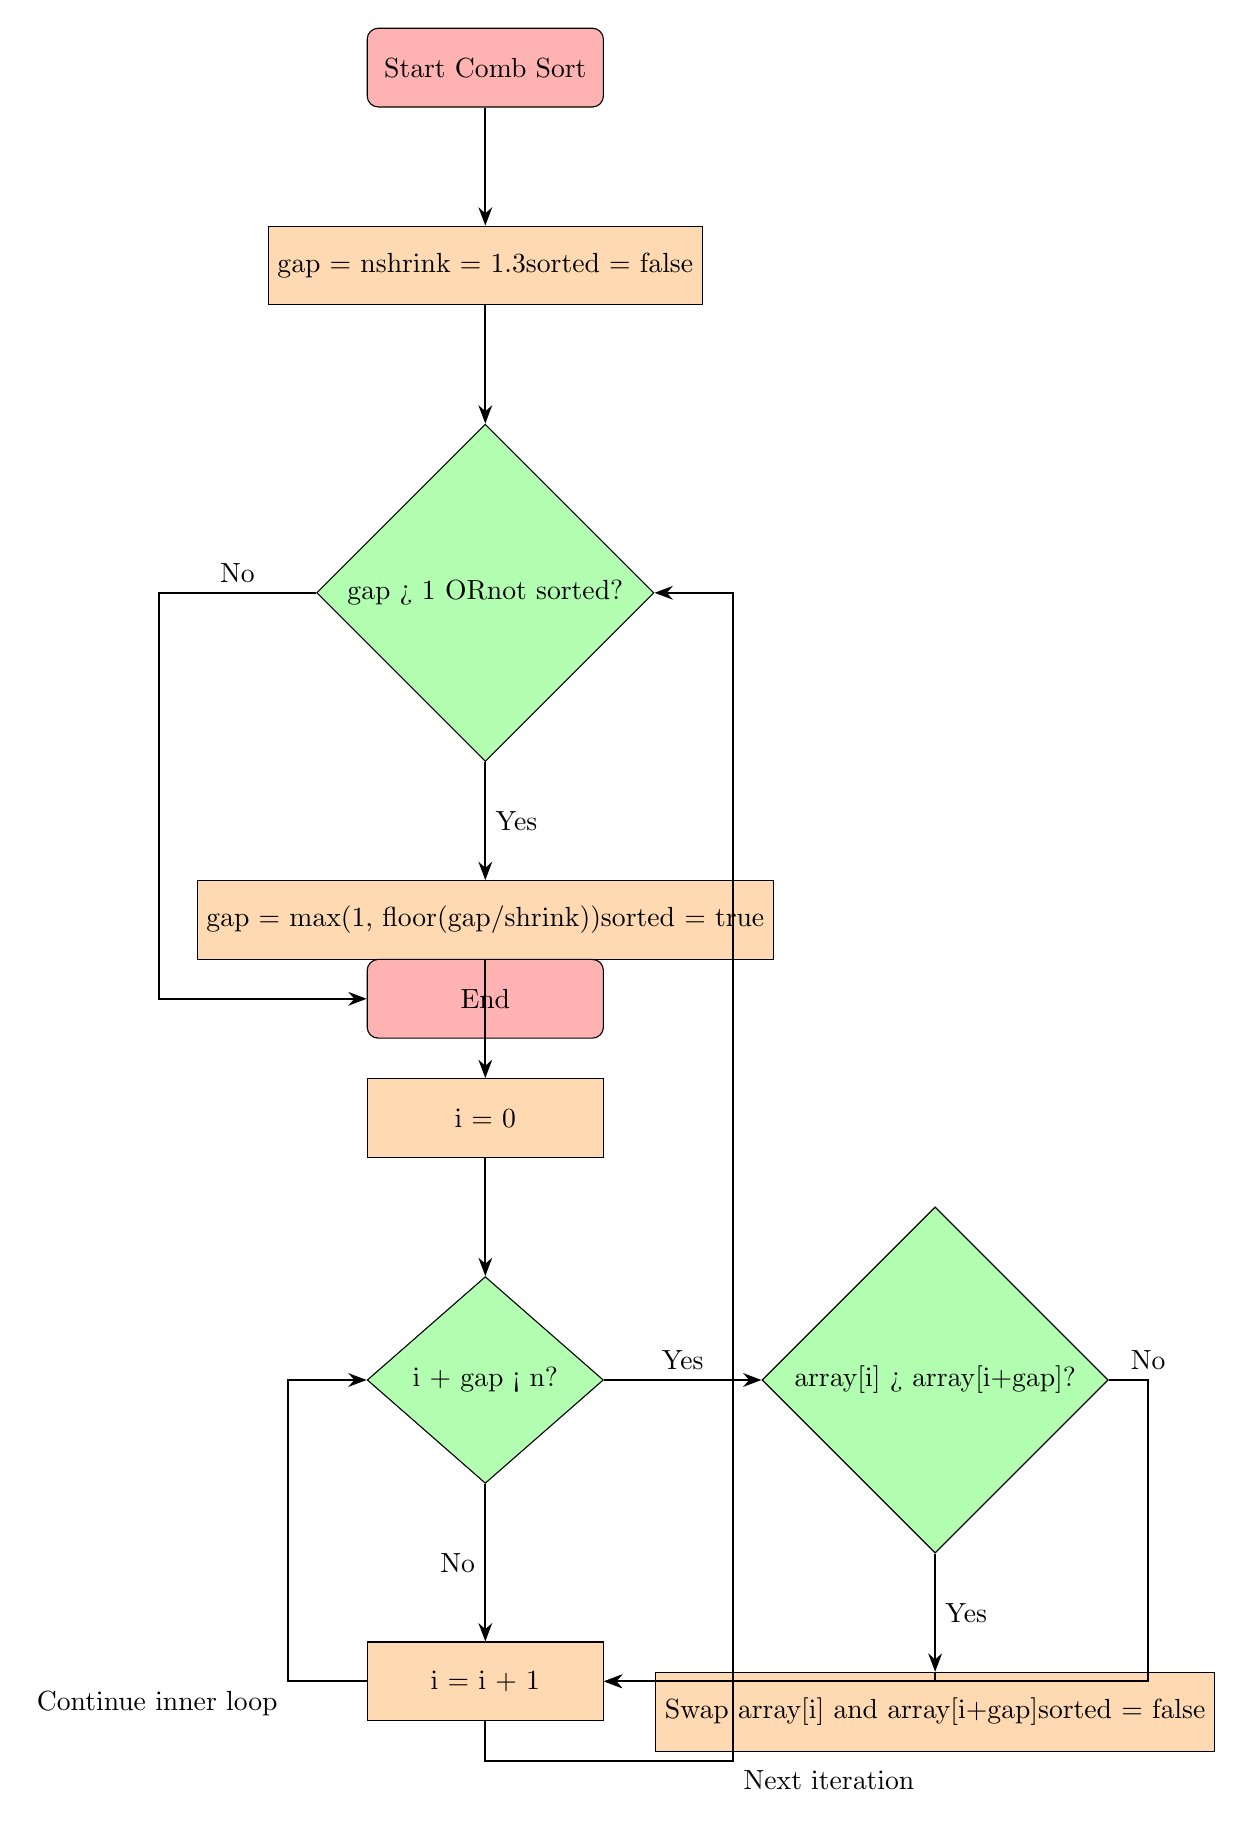
\begin{tikzpicture}[node distance=1.5cm]

% Main algorithm flow
\node (start) [startstop] {Start Comb Sort};
\node (init) [process, below=of start] {gap = n\\shrink = 1.3\\sorted = false};
\node (dec1) [decision, below=of init] {gap > 1 OR\\not sorted?};
\node (update) [process, below=of dec1] {gap = max(1, floor(gap/shrink))\\sorted = true};
\node (init_i) [process, below=of update] {i = 0};
\node (dec2) [decision, below=of init_i] {i + gap < n?};

% Inner loop - comparison and swap
\node (dec3) [decision, right=2cm of dec2] {array[i] > array[i+gap]?};
\node (swap) [process, below=of dec3] {Swap array[i] and array[i+gap]\\sorted = false};
\node (increment) [process, below=2cm of dec2] {i = i + 1};
\node (stop) [startstop, below=2.5cm of dec1] {End};

% Connections - main flow
\draw [arrow] (start) -- (init);
\draw [arrow] (init) -- (dec1);
\draw [arrow] (dec1) -- node[right] {Yes} (update);
\draw [arrow] (update) -- (init_i);
\draw [arrow] (init_i) -- (dec2);

% Connections - inner loop
\draw [arrow] (dec2) -- node[above] {Yes} (dec3);
\draw [arrow] (dec3) -- node[right] {Yes} (swap);
\draw [arrow] (swap) |- (increment);

% Connections - no swap path
\draw [arrow] (dec3.east) -- ++(0.5,0) node[above] {No} |- (increment.east);

% Connections - loop back
\draw [arrow] (increment.west) -| node[below left] {Continue inner loop} ([xshift=-1cm]dec2.west) -- (dec2.west);

% Connections - exit conditions
\draw [arrow] (dec2.south) -- node[left] {No} (increment.north);
\draw [arrow] (increment.south) -- ++(0,-0.5) -| node[below right] {Next iteration} ([xshift=1cm]dec1.east) -- (dec1.east);

\draw [arrow] (dec1.west) -- node[above] {No} ++(-2,0) |- (stop.west);

\end{tikzpicture}
\end{document}
